% Generated from report/DRAFT.md by build_report.py.
\section{Introduction and research question}\label{introduction-and-research-question}

A table-analysis assistant should translate a question into the right population, measure, aggregation and display, then explain what the computed evidence supports. These requirements are distinct. For example, independently recomputing revenue under a declared date filter does not establish that the filter selects the requested month. Correctly citing an hourly mean does not establish that the hour represents commuting activity.

We study whether verification and bounded correction improve the reliability of a locally deployed language-model agent under a fixed resource budget. The three task tiers are explicit statistical questions, specified visualizations and open-ended exploration. Our practical priority is reliable statistics and charts; exploration remains part of evaluation, with its limitations and failures reported.

The system follows the interaction between reasoning and tools exemplified by ReAct {[}1{]} and bounded feedback/refinement approaches such as Self-Refine {[}2{]}. LIDA {[}3{]} motivates treating visualization as a multi-stage analysis task, while DSBench {[}4{]} provides broader context for evaluating data-science agents. Our contribution is an implemented, instrumented comparison in a restricted single-table setting, rather than a new general reasoning algorithm.

The main question is: \textbf{under the same model, inputs and resource caps, does verification with bounded repair improve task outcomes enough to justify its latency and token cost?} We separately assess whether a failure is detected, whether a correction succeeds and whether a previously usable result regresses.

\section{System}\label{system}

\subsection{Workflow and common components}\label{workflow-and-common-components}

A Streamlit application accepts one CSV, a natural-language question and optional field documentation. Profiling records types, missingness, examples, numerical summaries and a CSV hash. LangGraph maintains the plan, generated program, execution artifacts, report candidates, feedback and budgets.

The plan declares conversions, derived fields, filters, missing-value policy, grouping, aggregation, sorting, output limits and chart specifications. Repairs of structurally and field-valid plans use sparse field updates against the saved plan: omitted/null fields retain their values, removals are explicit, and the merged plan is revalidated. This reduces accidental omission without guaranteeing a correct edit. Initial planning and structurally invalid candidates still use a complete plan. It may link verbatim excerpts of the request to intended analyses. These links are a proposed coverage map; validating an excerpt does not establish that every requirement is covered. An essential ambiguity can trigger a clarification. The CLI and evaluation runner support one prewritten reply in the same run without resetting the budget.

\begin{figure}[htbp]\centering
\pandocbounded{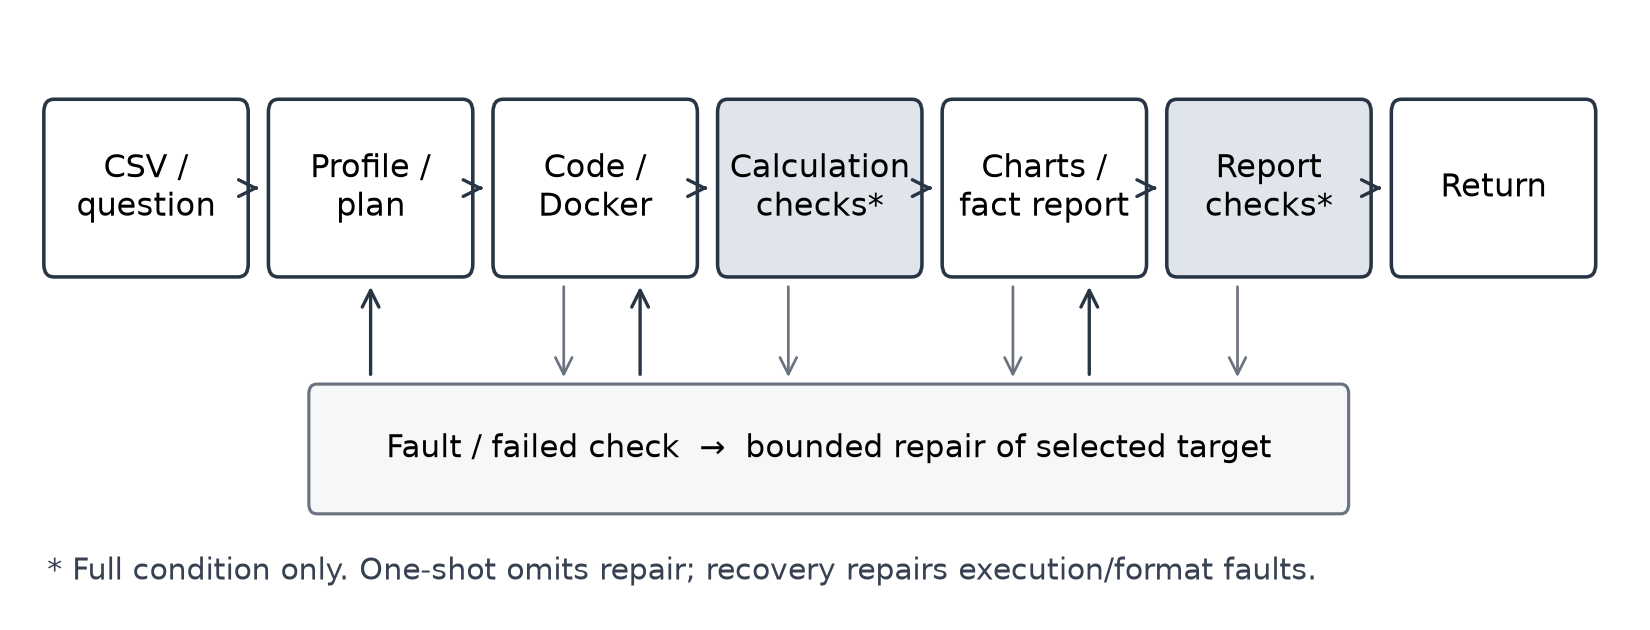
\includegraphics[keepaspectratio,alt={Workflow of the full condition; the caption identifies omitted stages in the two baselines.}]{../../docs/system-workflow.png}}
\par\smallskip
\begin{minipage}{\linewidth}\small
\textbf{Figure 1.} Full workflow, with verification stages shaded. One-shot omits verification and repair; error recovery omits verification and permits execution/format repair. Repairs target the plan, code or report within shared budgets.
\end{minipage}
\end{figure}

Shared preprocessing applies declared conversions and derived fields, then prepares an independent input frame for each analysis with its declared filters and missing-value rules. Aggregate inputs retain all-missing groups so undefined means and zero valid counts remain representable. The model generates aggregation, output columns, sorting and limits from these inputs. Both the raw generated program and the effective script are saved with hashes and preparation row counts. All conditions share this machinery; preprocessing implements the plan and does not certify its suitability.

Generated code runs only inside a non-root Docker container, with network disabled, read-only inputs and root filesystem, a writable artifact directory, and time/resource caps. Matplotlib renders bar, line, scatter and histogram charts from saved tables. Actual artist arrays, labels and histogram bins are retained for checking. Multi-table joins, predictive modeling and causal inference are outside scope.

\subsection{Reports and evidence}\label{reports-and-evidence}

The model selects one to four computed fact IDs for each of at most three findings and may add a short qualitative interpretation. A compiler inserts the measure, group labels, values and valid counts in fixed positions and attaches resolvable references. A mean based on one valid observation gets an explicit caution; empty outputs and undefined statistics remain explicit. The current catalog exposes up to twelve preview rows plus numerical extrema witnesses from the complete saved output. Full tables remain available; a limited output does not establish a population extremum.

The latest interface adds compiled maximum/minimum witnesses, extrema comparisons and observation-count ranges. Ties are explicit and statements are scoped to the complete saved output. Scalar missing-entry counts with matching declared filters may be compared across fields, explicitly as counts rather than rates. A narrow runtime wording rule rejects free-form ranking/comparison/significance terms in findings and requests computed facts instead; conditional limitations remain possible. It does not recognize all paraphrases or establish general semantic correctness.

A short decoding pattern excludes ASCII digits and braces from qualitative fields. Runtime validation additionally rejects Unicode number characters and terminal controls. Numeric field names and category labels remain usable through bound facts. The model also sees a minimal example with an actual fact ID and an empty interpretation. Invalid responses, full parser diagnostics and billed usage are saved; repair feedback contains a bounded set of field locations and errors. The program does not strip numbers from invalid responses or count them as successful reports.

This interface authenticates a fact\textquotesingle s location in computed output. It does not establish that the output is correct or that the model\textquotesingle s interpretation is true. It can also leave awkward prose when the model attempts a numerical sentence without its number; the development results explicitly retain this failure mode.

\subsection{Verification, repair and budgets}\label{verification-repair-and-budgets}

Independent verification reconstructs supported sums, means, counts, missing counts, ratios and non-grouped Pearson correlations with separate CSV/math routines. It checks grouping, valid counts, sorting and chart/table agreement without reusing the pandas preprocessing helpers. Complete numeric raw observations and unambiguous sorted subsets have additional checks. Unsupported sampling, ambiguous subset ties and unsupported operations remain uncovered.

Narrow checks assess selected request constraints. These include explicit named scalar-sum requests, certain single-month requests, and a narrow English Top-K form with actual column names. The ranking check validates the named statistic/group, limit, primary value direction and explicitly requested tie order; ambiguous, negated, weighted or within-group forms remain outside this rule. For an untyped ISO date range, the current checker independently compares actual membership against the requested calendar month, holding other declared filters fixed. Matching membership passes for that snapshot; extra or omitted rows fail. Missing or unsupported date evidence remains uncovered. This replaces a conservative rejection of every untyped range, and does not establish general lexical-date safety or natural-language request verification.

The full condition checks calculations immediately after successful execution, before spending on charts and report drafting. After drafting, deterministic checks compare chart artifacts, resolve report facts and apply narrow wording rules. If no deterministic failure remains, a separate call to the same model assesses each finding, limitation and whole-request coverage; otherwise semantic review is deferred until repair. These stages count as one logical verification invocation per candidate, with separate active durations. A completed or failed report review cannot be reused for a free retry. A calculation-only inspection cannot promote a candidate to a reviewed final report.

Feedback can target the plan, code or report. New plans require fresh code and execution; report-only repair can reuse the saved calculations. Previous attempts and failures remain available. The controller stops at exhausted budgets, insufficient reservation or repeated unresolved errors. Failed tools and model outputs consume the same caps as successful ones.

Current additional plan/code/chart review issues must name an actual artifact location and quote its content. Report statements retain their own required verdicts, and report-repair guidance supplies available computed comparisons. A report quote cannot serve as an actual chart-label quote. This constrains feedback provenance and routing, while leaving the reviewer\textquotesingle s error judgment heuristic.

Each run permits at most twelve tool invocations, three corrections and 100,000 cumulative model tokens. Model output is capped at 6,144 tokens with a 16,384-token context. All stages use Qwen3.5-9B Q4 with thinking disabled, temperature 0.7, top\_p 0.8, top\_k 20, repeat penalty 1 and presence penalty 1.5; the initial seed is 42. The evaluation host is an Apple M5 with ten CPU cores and 24 GiB memory; execution containers use two CPUs and a 2 GiB limit. Model/image digests, dependencies and hardware are recorded in each run.

\texttt{checks\_passed} means applicable automated checks and model review reported no unresolved failure. It is not a human whole-task pass, and uncovered checks remain visible.

\section{Data and evaluation}\label{data-and-evaluation}

\subsection{Data and conditions}\label{data-and-conditions}

{\def\LTcaptype{none} % do not increment counter
\begin{table}[htbp]\centering
\begin{tabular}{@{}
  >{\raggedright\arraybackslash}p{(\linewidth - 4\tabcolsep) * \real{0.2300}}
  >{\raggedleft\arraybackslash}p{(\linewidth - 4\tabcolsep) * \real{0.1300}}
  >{\raggedright\arraybackslash}p{(\linewidth - 4\tabcolsep) * \real{0.6400}}@{}}
\toprule\noalign{}
\begin{minipage}[b]{\linewidth}\raggedright
Dataset
\end{minipage} & \begin{minipage}[b]{\linewidth}\raggedleft
Recorded rows
\end{minipage} & \begin{minipage}[b]{\linewidth}\raggedright
Analysis scope
\end{minipage} \\
\midrule\noalign{}
UCI Online Retail {[}5{]} & 541,909 & Transactions; positive-sales tasks specify cancellation, quantity, price and date constraints; revenue is Quantity × UnitPrice. \\
UCI Bike Sharing {[}6{]} & 17,379 & Hourly table; weather normalization and category meanings use the supplied documentation. \\
UCI Adult {[}7{]} & 48,842 & Combined supplied files; unweighted sample descriptions unless weighting is explicitly requested. \\
\bottomrule
\end{tabular}
\end{table}
}

Source URLs, licenses, preprocessing and hashes are recorded locally; the dataset pages list CC BY 4.0. The study concerns new tasks on three known datasets, not unseen-domain generalization.

{\def\LTcaptype{none} % do not increment counter
\begin{table}[htbp]\centering
\begin{tabular}{@{}
  >{\raggedright\arraybackslash}p{(\linewidth - 2\tabcolsep) * \real{0.2400}}
  >{\raggedright\arraybackslash}p{(\linewidth - 2\tabcolsep) * \real{0.7600}}@{}}
\toprule\noalign{}
\begin{minipage}[b]{\linewidth}\raggedright
Condition
\end{minipage} & \begin{minipage}[b]{\linewidth}\raggedright
Behavior
\end{minipage} \\
\midrule\noalign{}
One-shot & One plan/program/report workflow without correction or explicit verification. \\
Error recovery & Allows execution and format recovery, without independent verification or semantic review. \\
Full & Adds programmatic checks, same-model semantic review and bounded correction. \\
\bottomrule
\end{tabular}
\end{table}
}

Conditions share data, documentation, profiling, preprocessing, report interfaces, libraries and resource caps. The tested agent\textquotesingle s same-model review cost is included in its full condition. One-time external reference-audit cost is recorded separately and is not part of the agent-condition comparison. Neither the agent nor its same-model reviewer receives the evaluation reference answers. The comparison measures the verification package under a cap; it does not isolate the effect of one checker.

\subsection{Frozen formal protocol}\label{frozen-formal-protocol}

The protocol contains six development tasks and thirty held-out base tasks: twelve explicit questions, twelve visualization tasks and six explorations. Twelve variants add numeric strings, mixed unambiguous dates or missing entries. Including variants, the frozen grid is forty-two inputs × three conditions × two repeats, or 252 runs. All forty-two inputs expect a direct substantive answer. Incidental clarification is recorded, but this grid does not empirically test the supported prewritten clarification-response workflow.

The proposal\textquotesingle s independent-human reference/family review has been revised to an external model-assisted audit using SudoCode\textquotesingle s Chat Completions-compatible endpoint, configured as \texttt{gpt-6.1-sol}. For each deterministic task, the auditor sees the question, documentation, columns and three formatting examples, but no existing answer, reference implementation or agent output. It generates independent code for network-disabled local execution and complete-table comparison. Exploration tasks receive scope/scoreability review without a fabricated unique answer. The relay\textquotesingle s returned identifier does not independently verify model identity; correlated model errors remain possible. The pre-test audit also flagged one retained chart prompt\textquotesingle s "GBP per line" axis wording: it explicitly requests the unweighted mean of UnitPrice across transaction lines, but the documented measure is GBP per unit. The numerical reference follows that mean, and pre-test rater guidance clarifies the documented unit; the ambiguity remains a limitation of that item. Audit tokens and failures are recorded separately, with dollar cost unknown because pricing is not configured. The final candidate required fifty-five saved responses, including incomplete programs for two tasks, their explicit supplements and one code-array transport adaptation. All forty deterministic reference tables matched; eight exploratory tasks received scope review. Across all pre-test revisions, 174 responses report 459,903 input and 151,359 output tokens, with two responses lacking token measurements. These audit calls are separate from Qwen outcomes and condition costs.

A question-text-only family check initially missed overlap. We therefore reviewed actual attempted development plans, including failed attempts and early/application runs. Conflicting model judgments prompted a written operational boundary: shared primitives alone do not establish rehearsal, while the same substantive target/template with altered dates, subsets, group labels or display remains exposed. Revisions removed rehearsed weather associations, temporal coverage, Adult age/education and capital-gain comparisons, general category-composition exploration, and direct supplied-weight summaries potentially exposed through failed ratio intermediates. No Qwen formal-test outputs informed these revisions. The revised test catalog has eight conservative connected families; exploratory tasks can connect several narrower tests, which remain together with their variants for resampling. This is new-request evaluation on familiar data and operations, with few family-level units and limited inferential strength. The revised audit and source/configuration freeze preceded formal inference. All 252 runs are complete; human scoring and adjudication of the amended sample below are complete.

Numerical tables use exact agreement for categories/counts and floating-point tolerances of relative 1e-4 and absolute 1e-6. A numerical match means that at least one saved table in the selected candidate agrees with the complete reference, including required counts, grouping and ordering. It does not certify additional analyses or a correct textual answer. A missing selected output fails this numerical metric; earlier matching computations remain separate candidate evidence. Explicit tasks also require correct scope and explanation. Visualization scoring covers data, type, axes/units/labels and legibility, each on a 0-\/-2 scale; a pass requires correct data, explicit constraints and at least 6/8. Up to three exploratory findings receive correctness, grounding and usefulness scores of 0-\/-2. A response with no substantive finding receives zero; an absent extra finding is not automatically penalized.

Automatic analysis retains all 252 runs, averaging repeats within each input. Descriptive paired intervals resample task families within each dataset while retaining clean/variant dependence. Automatic numerical outcomes, variants and costs are reported separately from human whole-task judgments.

\subsection{Post-hoc human-sample amendment}\label{post-hoc-human-sample-amendment}

After inspecting automatic outcomes, on 18 November we reduced full-grid double rating to twenty-seven outputs to fit rater availability. This post-hoc amendment fixed selection rules before sampling. All forty-two frozen inputs, including variants, are eligible. Dataset order is Adult, Bike, Retail; tier order is explicit, exploration, visualization; task IDs are sorted within each stratum. Python\textquotesingle s \texttt{random.Random(42)} selects one input per stratum, retaining all three conditions at fixed repeat zero. Selection reads metadata only, with no outcome-based replacement or reseeding. The saved manifest binds candidates, selection, source hashes and anonymous evidence.

Both teammates independently rated the same anonymous sample under the original rubric. Twelve outputs had final reports; fifteen did not. Multiple exploratory findings yielded thirty-seven rows per rater. Initial sheets were blank; absent-output zeros required human confirmation. After receiving both initial ratings, we assigned final adjudication to Liu He, who developed the system. He chose seven disputed scores through an interface showing anonymous evidence and both ratings, with no preselected score. He is not an independent third-party adjudicator. Original returns and separate adjudication records preserve initial agreement; agreed scores were unchanged.

Each tier/condition has only three outputs, potentially sharing families. Human pass counts, rubric means (averaging findings within output) and agreement describe this sample only. The other 225 outputs stay unrated. We make no imputation, full-grid human pass-rate estimate, human bootstrap interval, robustness or repeat-stability inference. Sample completion passed a separate gate; the original full-grid human gate remains incomplete.

\section{Development evidence}\label{development-evidence}

Development informed the system and task-family audit; repeatedly inspected requests are excluded from formal outcome claims. Complete runs, failed attempts and version-specific costs remain in the development evidence ledger, rather than being pooled across changing implementations.

Development exposed four design concerns: a plan can violate request scope while passing recomputation; a replacement plan can lose a needed derivation; valid calculations can fail the report contract or output cap; and same-model review can accept unsupported interpretations. These observations motivated sparse plan updates, earlier calculation checks, fact-bound reports and narrow request checks. The last complete six-task development comparison had eighteen terminal runs, only two matching selected tables among four explicit/chart tasks in each condition, and no human whole-task scores. A subsequent prespecified two-task follow-up retained one corrected ranking table and one unresolved date-filter failure. These diagnostics did not establish held-out improvements.

A separate real-Chrome integration uploaded a six-row CSV and requested total rentals, valid count and a weather bar chart. It completed without repair in 102.17 seconds and 18,481 tokens: total 152 over six observations; Clear 67/3, Misty 28/1 and Rain 57/2. The actual HTTP export matched all seventy-one ZIP entries and excluded the raw CSV. Automation fetches that registered resource without clicking Download because Chrome\textquotesingle s native Save As dialog cannot be completed by the connector. Native dialog completion is outside this check. The later shared-export refactor did not alter the analysis logic.

\section{Results: full automatic grid and human sample}\label{results-full-automatic-grid-and-human-sample}

The complete 252-run grid finished without selective retries. Integrity checks verified 17,829 saved run files, fixed-grid membership, source/input/environment fingerprints, terminal ledgers and budgets. An initial direct-script launch failed at import before cohort creation or model calls; the module entry ran the unchanged grid, with both logs retained. The following results include failures and budget stops. Sections 5.1-5.4 describe automatic measurements of selected outputs; Section 5.5 reports the separate human sample.

\subsection{Numerical tables and report availability}\label{numerical-tables-and-report-availability}

{\def\LTcaptype{none} % do not increment counter
\begin{table}[htbp]\centering
\begin{tabular}{@{}
  >{\raggedright\arraybackslash}p{(\linewidth - 6\tabcolsep) * \real{0.4000}}
  >{\raggedleft\arraybackslash}p{(\linewidth - 6\tabcolsep) * \real{0.2000}}
  >{\raggedleft\arraybackslash}p{(\linewidth - 6\tabcolsep) * \real{0.2000}}
  >{\raggedleft\arraybackslash}p{(\linewidth - 6\tabcolsep) * \real{0.2000}}@{}}
\toprule\noalign{}
\begin{minipage}[b]{\linewidth}\raggedright
Selected numerical table
\end{minipage} & \begin{minipage}[b]{\linewidth}\raggedleft
One-shot
\end{minipage} & \begin{minipage}[b]{\linewidth}\raggedleft
Error recovery
\end{minipage} & \begin{minipage}[b]{\linewidth}\raggedleft
Full
\end{minipage} \\
\midrule\noalign{}
Explicit questions & 21/44 (47.7\%) & 26/44 (59.1\%) & 27/44 (61.4\%) \\
Specified charts & 5/28 (17.9\%) & 12/28 (42.9\%) & 14/28 (50.0\%) \\
\bottomrule
\end{tabular}
\par\smallskip
\begin{minipage}{\linewidth}\small
\textbf{Table 1.} Complete-table numerical agreement with the externally audited reference. A match requires at least one saved table in the selected candidate to agree with the complete reference; it does not certify every extra analysis. Each denominator includes all two-repeat runs for that tier. A missing selected report scores as no matching final table under the frozen evaluator, even if an earlier computation matched. Explicit answer semantics, chart legibility and exploration quality require human ratings.
\end{minipage}
\end{table}
}

{\def\LTcaptype{none} % do not increment counter
\begin{table}[htbp]\centering
\begin{tabular}{@{}
  >{\raggedright\arraybackslash}p{(\linewidth - 6\tabcolsep) * \real{0.4000}}
  >{\raggedleft\arraybackslash}p{(\linewidth - 6\tabcolsep) * \real{0.2000}}
  >{\raggedleft\arraybackslash}p{(\linewidth - 6\tabcolsep) * \real{0.2000}}
  >{\raggedleft\arraybackslash}p{(\linewidth - 6\tabcolsep) * \real{0.2000}}@{}}
\toprule\noalign{}
\begin{minipage}[b]{\linewidth}\raggedright
A selected report was available
\end{minipage} & \begin{minipage}[b]{\linewidth}\raggedleft
One-shot
\end{minipage} & \begin{minipage}[b]{\linewidth}\raggedleft
Error recovery
\end{minipage} & \begin{minipage}[b]{\linewidth}\raggedleft
Full
\end{minipage} \\
\midrule\noalign{}
Explicit questions & 24/44 & 32/44 & 30/44 \\
Specified charts & 8/28 & 19/28 & 19/28 \\
Open exploration & 1/12 & 9/12 & 5/12 \\
\bottomrule
\end{tabular}
\par\smallskip
\begin{minipage}{\linewidth}\small
\textbf{Table 2.} Availability includes retained candidates from failed runs and does not imply correctness. Plotted arrays agreed with the task reference in 5/28 one-shot runs, 12/28 error recovery runs, 14/28 full runs. This does not evaluate unit semantics, explanation or display readability.
\end{minipage}
\end{table}
}

\subsection{All-run resource cost}\label{all-run-resource-cost}

Table 3 includes every run, including failures. Full used 2.59 times the one-shot model tokens and 1.60 times the recovery tokens. Figure 2 separates token and elapsed-time costs by tier; timing is descriptive because the runs were not isolated cold-start trials.

{\def\LTcaptype{none} % do not increment counter
\begin{table}[htbp]\centering
\begin{tabular}{@{}
  >{\raggedright\arraybackslash}p{(\linewidth - 6\tabcolsep) * \real{0.4000}}
  >{\raggedleft\arraybackslash}p{(\linewidth - 6\tabcolsep) * \real{0.2000}}
  >{\raggedleft\arraybackslash}p{(\linewidth - 6\tabcolsep) * \real{0.2000}}
  >{\raggedleft\arraybackslash}p{(\linewidth - 6\tabcolsep) * \real{0.2000}}@{}}
\toprule\noalign{}
\begin{minipage}[b]{\linewidth}\raggedright
Measurement per condition
\end{minipage} & \begin{minipage}[b]{\linewidth}\raggedleft
One-shot
\end{minipage} & \begin{minipage}[b]{\linewidth}\raggedleft
Error recovery
\end{minipage} & \begin{minipage}[b]{\linewidth}\raggedleft
Full
\end{minipage} \\
\midrule\noalign{}
Accounted model tokens, total & 888,793 & 1,433,807 & 2,299,457 \\
Accounted tokens, mean per run & 10,581 & 17,069 & 27,374 \\
Elapsed seconds, mean per run & 58.7 & 84.9 & 142.5 \\
Corrections, mean per run & 0.00 & 1.05 & 1.39 \\
\bottomrule
\end{tabular}
\par\smallskip
\begin{minipage}{\linewidth}\small
\textbf{Table 3.} All eighty-four runs per condition contribute, including failures. Balanced two-repeat coverage makes the run mean equal to averaging repeats within each input first. Across the grid, 913 model calls used 4,622,057 accounted tokens. Every call reported token usage; none required an unknown-usage reservation charge. External audit costs are excluded.
\end{minipage}
\end{table}
}

\begin{figure}[htbp]\centering
\pandocbounded{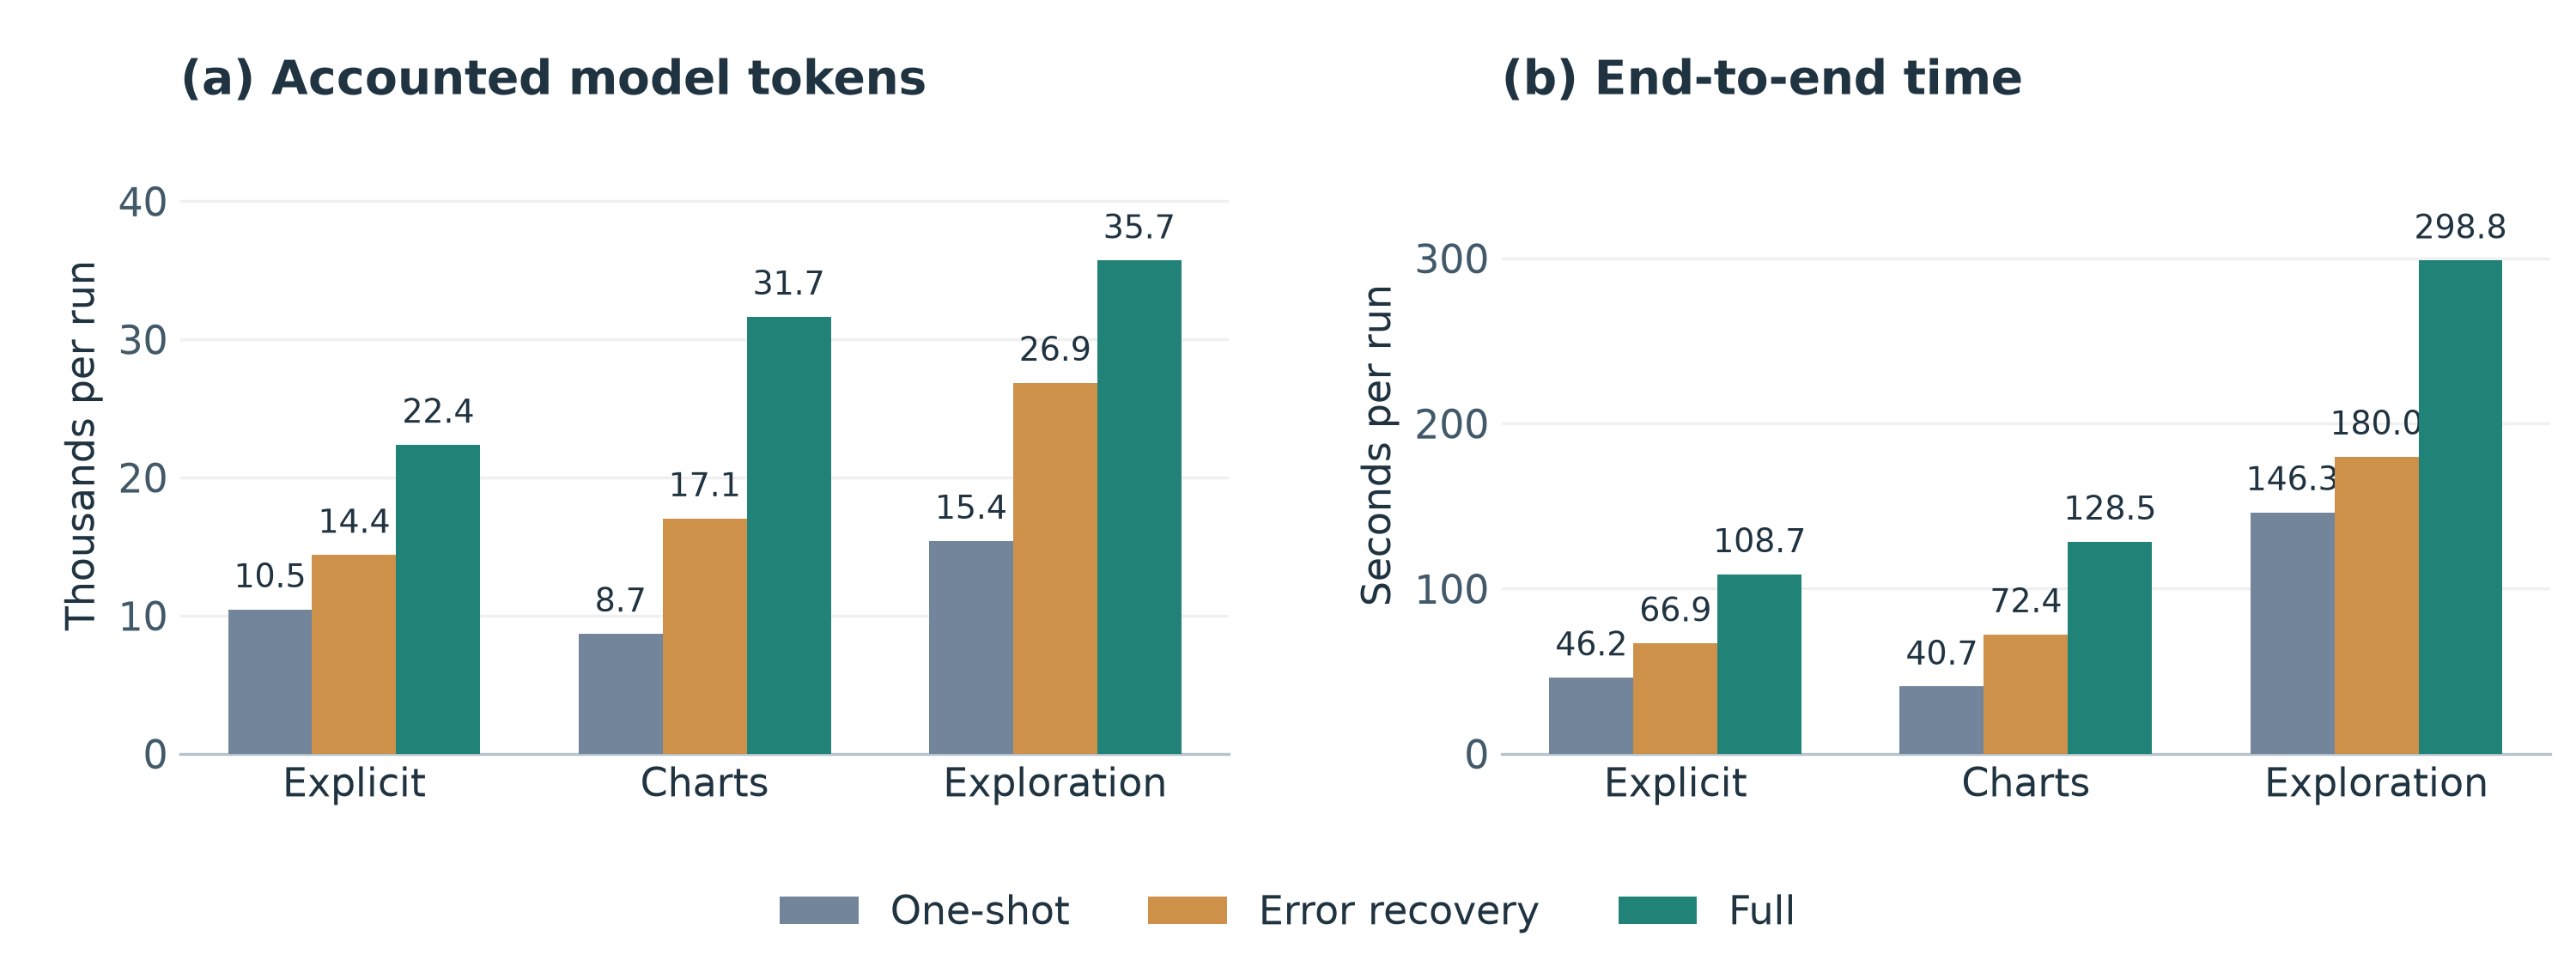
\includegraphics[keepaspectratio,alt={All-run token and elapsed-time costs by tier and condition.}]{../../docs/formal-v7-costs.png}}
\par\smallskip
\begin{minipage}{\linewidth}\small
\textbf{Figure 2.} Costs include failed workflows. Sequential ordering, cache state and concurrent local documentation/source checks prevent a causal cold-start latency comparison. Server loading, prompt/generation computation and client-call wall time are separately retained with measurement counts. Process RSS excludes Metal allocations and the Docker VM.
\end{minipage}
\end{figure}

\subsection{Candidate transitions and variants}\label{candidate-transitions-and-variants}

Among full-condition deterministic runs with a scored initial candidate, 13/44 initial candidates without a matching table, including failed or absent computations, led to a matching selected final output, while 0/28 initially matching tables ended without a matching final output. Every deterministic run had a scored initial candidate. These are numerical-candidate transitions, not human task-level recovery: an initial matching table may never have yielded a usable report.

Paired variants compare each perturbed input with its clean partner after averaging repeats. Missing-value variants can change the valid reference answer. Numeric strings alter representation and may be inferred correctly by pandas; mixed dates remain unambiguous. Full paired results are retained in the secondary analysis, with reused clean tasks and shared families explicitly dependent.

{\def\LTcaptype{none} % do not increment counter
\begin{table}[htbp]\centering
\begin{tabular}{@{}
  >{\raggedright\arraybackslash}p{(\linewidth - 6\tabcolsep) * \real{0.4000}}
  >{\raggedleft\arraybackslash}p{(\linewidth - 6\tabcolsep) * \real{0.2000}}
  >{\raggedleft\arraybackslash}p{(\linewidth - 6\tabcolsep) * \real{0.2000}}
  >{\raggedleft\arraybackslash}p{(\linewidth - 6\tabcolsep) * \real{0.2000}}@{}}
\toprule\noalign{}
\begin{minipage}[b]{\linewidth}\raggedright
Variant minus clean numerical match
\end{minipage} & \begin{minipage}[b]{\linewidth}\raggedleft
One-shot
\end{minipage} & \begin{minipage}[b]{\linewidth}\raggedleft
Error recovery
\end{minipage} & \begin{minipage}[b]{\linewidth}\raggedleft
Full
\end{minipage} \\
\midrule\noalign{}
Numeric strings & -12.5 pp & +0.0 pp & +0.0 pp \\
Missing values & +0.0 pp & +0.0 pp & +0.0 pp \\
Mixed dates & +0.0 pp & -25.0 pp & -50.0 pp \\
\bottomrule
\end{tabular}
\par\smallskip
\begin{minipage}{\linewidth}\small
\textbf{Table 4.} Descriptive pair means over four numeric-string, six missing-value and two mixed-date pairs. Each clean/variant input has two repetitions; shared clean tasks and families do not create independent samples. These are differences in reference-match rates, not raw statistic changes or human task-quality differences.
\end{minipage}
\end{table}
}

Descriptive family-resampling intervals for full minus one-shot were +13.64 percentage points {[}4.55, 23.08{]} for explicit questions and +32.14 {[}22.73, 38.24{]} for charts. Against error recovery they were +2.27 {[}0, 4.55{]} and +7.14 {[}0, 13.33{]}. These 95\% intervals use 10,000 dataset-stratified family resamples with seed 42; repeated inputs and variants stay together. The selected families do not support broad population significance claims. Zero mean change for missing-value variants can mask opposing pair differences, while zero in any variant category can mean both inputs failed.

\subsection{Saved correction and failure cases}\label{saved-correction-and-failure-cases}

A Retail cancellation-count run initially summed Quantity instead of counting records. Independent calculation checks passed because the table agreed with that wrong plan. Same-model review identified the request mismatch, and one plan/code correction produced the complete reference-matching count table. This illustrates a request-level correction beyond arithmetic consistency, without establishing a human whole-answer pass.

A mixed-date Bike temperature-chart run never declared date conversion. Both saved candidates used textual date bounds and retained 496 July observations, whereas the parsed-year reference contains 744. Their means and counts agreed with independent recomputation of the declared plan but failed the task reference. Request coverage received a model pass; the aggregate semantic verdict failed, and repair repeated the date-filter error. This is a concrete limit of plan-relative checking and same-model diagnosis.

A workclass capital-loss/capital-gain ratio run failed all four execution attempts: the first used an unsupported pandas keyword, the second referenced an absent output column, and the final two repeated a nonexistent pandas constant. No report was selected. More generally, code/draft output-cap truncations numbered 2/2 for one-shot, 6/3 for recovery and 7/3 for full; full also recorded ten semantic-review model-call failures. These are overlapping stage diagnostics, including recovered failures, not a partition of terminal failures. All consumed resources remain in Table 3.

\subsection{Human sample and initial agreement}\label{human-sample-and-initial-agreement}

{\def\LTcaptype{none} % do not increment counter
\begin{table}[htbp]\centering
\begin{tabular}{@{}
  >{\raggedright\arraybackslash}p{(\linewidth - 6\tabcolsep) * \real{0.4000}}
  >{\raggedleft\arraybackslash}p{(\linewidth - 6\tabcolsep) * \real{0.2000}}
  >{\raggedleft\arraybackslash}p{(\linewidth - 6\tabcolsep) * \real{0.2000}}
  >{\raggedleft\arraybackslash}p{(\linewidth - 6\tabcolsep) * \real{0.2000}}@{}}
\toprule\noalign{}
\begin{minipage}[b]{\linewidth}\raggedright
Sample outcome
\end{minipage} & \begin{minipage}[b]{\linewidth}\raggedleft
One-shot
\end{minipage} & \begin{minipage}[b]{\linewidth}\raggedleft
Error recovery
\end{minipage} & \begin{minipage}[b]{\linewidth}\raggedleft
Full
\end{minipage} \\
\midrule\noalign{}
Explicit-task pass & 1/3 & 1/3 & 1/3 \\
Chart-task pass & 1/3 & 1/3 & 2/3 \\
Chart rubric mean (0-8) & 2.67 & 2.67 & 5.33 \\
Exploration correctness (0-2) & 0.00 & 1.89 & 1.33 \\
Exploration grounding (0-2) & 0.00 & 1.89 & 1.33 \\
Exploration usefulness (0-2) & 0.00 & 1.78 & 1.22 \\
Exploration total (0-6) & 0.00 & 5.56 & 3.89 \\
\bottomrule
\end{tabular}
\par\smallskip
\begin{minipage}{\linewidth}\small
\textbf{Table 5.} Adjudicated results for the fixed twenty-seven-output sample. Each tier/condition has three outputs. Explicit/chart passes combine human criteria with the frozen numerical, chart and protocol gates; they are not human scores alone. Exploration scores average findings within each output, then average the three outputs equally. Missing reports remain zero. The other 225 outputs have no human ratings.
\end{minipage}
\end{table}
}

All three conditions passed the same one sampled explicit task. Full passed two sampled chart tasks, versus one for each baseline, while its exploration mean was lower than recovery\textquotesingle s. The sampled explorations had zero, three and two available reports for one-shot, recovery and full; report absence contributes directly to these means. This sample does not establish general superiority, repeat stability or full-grid whole-task quality.

Before adjudication, twenty-three of twenty-seven outputs had identical required ratings. The disagreements were six usefulness scores across three exploration outputs and one chart-type score. Exploration usefulness agreed on 13/19 rows (68.4\%, mean absolute difference 0.316); chart type agreed on 8/9 (88.9\%, difference 0.111). Every other required dimension agreed exactly. Pooled required-cell agreement was 187/194 (96.4\%), including flags and missing-output zeros. Dependent findings and numerous zeros limit its interpretation; it is not an independent-sample reliability estimate or task-success rate. The seven final decisions and initial agreement are retained separately. No human bootstrap intervals or full-grid human estimates are reported.

\section{Discussion and limitations}\label{discussion-and-limitations}

The architecture separates three checks that are easy to conflate: whether code implements the plan, whether the plan implements the request and whether the explanation is supported. Common preprocessing improves enforcement of declared transformations, but can faithfully execute a wrong plan. Bound facts preserve labels and numbers, but the model can still write an unsupported interpretation or an incomplete sentence.

Same-model review can repeat assumptions, miss contradictions, propose incompatible repairs or route a report issue into unnecessary replanning. An internal pass cannot substitute for independent task assessment. Narrow deterministic checks improve specific covered cases while leaving unsupported requests explicit; they do not establish general verification.

The development sample is small, uses one repeat per cell and has been repeatedly inspected during implementation. It cannot establish held-out answer quality, exploration usefulness, human chart legibility or robustness. The initial model-assisted audit missed development/test overlap until actual attempted plans were supplied. Boundary judgments also varied across requests. The final model-assisted audit passed after these revisions; no human reference review or human-equivalent review accuracy is claimed. The eight connected test families, and only four exploration-bearing families, limit the strength of resampling intervals. Human assessment is a post-hoc sample with three outputs per tier/condition and team-member raters. Final adjudication by a system developer can introduce bias; the initial independent agreement is therefore reported separately. Metadata-only selection avoids deliberately choosing successful outputs, but does not make the amendment prospective or support full-grid quality claims. Sequential task/condition ordering, cache state and hardware load also limit causal latency comparisons. Local document rendering and source-portability checks ran during the grid; no controlled cold-start or isolated-host timing study is claimed. Process RSS measurements exclude Metal allocations and the Docker VM.

The frozen results support a limited conclusion: full verification increased selected numerical matches relative to one-shot generation on these inputs, with smaller gains over execution/format recovery and substantially higher token cost. Across all inputs, it yielded 54 selected reports versus 60 for error recovery; for exploration the counts were 5/12 versus 9/12. Additional review can consume budget or reject a candidate without producing a usable replacement. The human sample showed one additional chart pass for full, equal explicit passes and lower exploration scores than recovery. With only three outputs per tier/condition and developer adjudication, it does not establish broad whole-task improvement or that the extra cost is justified. Correlated errors between language models remain possible; numerical agreement cannot establish that the task itself is valid.

\section{Reproduction and completion}\label{reproduction-and-completion}

README covers installation and use; the evaluation guide covers freezing and scoring. The sample protocol and \texttt{scripts.human\_sample} preserve selection, original returns and the separate summary. Hashed run artifacts and resource ledgers remain local. Downloads exclude raw CSV by default. Both original human returns, the developer\textquotesingle s adjudication and the verified twenty-seven-output summary are retained separately. The report distinguishes full-grid automatic evidence from sample human judgments.
